\subsection{Data Acquisition as Graph Crawling}\label{section:graph_to_website}
\begin{toappendix}
	\subsection{Data Acquisition as Graph Crawling}
\end{toappendix}

We complete our modeling of Web data acquisition as an instance of the
graph crawling problem by detailing the graph~$G$, the target subset
$V^*$, and the edge labeling function~$\lambda$. The choice of $\lambda$ will turn out to be crucial for the performance of our approach.

We identify pages by their URL and fix $r$, the website root, as the start of the crawl.
Next, we need to identify which pages belong to the website graph. Lacking a commonly agreed definition of a website's boundary~\cite{senellart2005identifying,alshukri2010website}, we use a pragmatic approach. A~URL is considered to be part of the same website as the root $r$ if \emph{its hostname} (the part of the URL which is after the scheme but before the path, with a potential ``www.'' prefix excluded) \emph{is a subdomain of the hostname of~$r$}.
$V$ contains all such URLs. For instance, if $r$ is \url{https://www.A.B.com/index.php}, the URLs \url{https://www.A.B.com/folder/content.php} and \url{https://www.C.A.B.com/page.html} are part of $V$, but \url{https://www.B.com/page.php} and \url{https://edbticdt2026.github.io/?contents=EDBT_CFP.html} are not.\footnote{The reason for the special handling of a ``www.'' prefix is that many (but not all\dots) websites use it as a prefix for the domain name of the
	Web server.} An edge $(u,v) \in E$ exists if $u$ links to $v$~via HTML
tags like \texttt{<a>}, \texttt{<area>},\texttt{<iframe>}.

Since our goal is to find SDs,
target pages are those whose \emph{Multipurpose Internet Mail
	Extensions} (MIME) type is in a
\emph{user-defined} list (e.g., 
{\small\verb|text/csv|}, {\small\verb|application/pdf|},
{\small\verb|application/vnd.ms-excel|}).
Non-target types include {\small\verb|text/html|},
{\small\verb|video/*|}, {\small\verb|audio/*|}, {\small\verb|image/*|}, etc. 
The MIME type can be obtained via HTTP HEAD requests; to generalize to other content than SDs, 
any other target MIME type set can be used. The full list of MIME types
we use 
is in~\cite{github_repository}.

To each edge $e$, the edge labeling function $\lambda$ associates as label $\lambda(e)$ the \textbf{tag path}
derived from the HTML page's DOM structure~\cite{DOM}, the standard tree-based representation of an HTML page.
The tag path includes the \textbf{full path of HTML tags from the root 
to the hyperlink tag} (\texttt{a}, \texttt{area}, \texttt{iframe}, etc.), along with class and id attributes
describing additional structural and styling information. For example, a
label might be ``\texttt{html} \texttt{body} \texttt{div\#main}
\texttt{ul.datasets} \texttt{li} \texttt{a}'', where `\texttt{\#}' prefixes
the HTML ID, and `\texttt{.}' indicates a class. This labeling makes it very likely that \emph{links labeled with similar tag paths lead to similar content types}, even across different webpages of the same website. Figure~\ref{fig:tag_paths_example} zooms within an HTML page. It shows five tag paths (the tags are omitted for readability), leading to: a text paragraph, an image and 3 hyperlinks to other pages (1 target, and~2~HTML pages). 
$\lambda$ captures exactly the tag paths leading to each hyperlink.
We consider two cost functions $\omega$: \begin{inparaenum}[(i)] \item counting HTTP requests, $\omega(u)$$=$$1$ for all $u$$\in$$V$; \item measuring the exchanged data volume, especially data volume the crawler receives with $\omega(u)$ as the page size, which is, in theory, unbounded. \end{inparaenum}
We also account for the cost $c$ of \emph{determining if a vertex is
	in~$V^*$}, typically via an HTTP HEAD request. If $\omega$ counts
requests, then $c(u)$$=$$1$; if $\omega$ measures volume, $c(u)$ is based on
HEAD response size (much smaller than $\omega(u)$). Sec.~\ref{subsection:url_classifier} discusses a MIME type prediction method, resulting in a small, amortized $c$ cost, which we can view as constant.

\begin{figure}
	\centering
	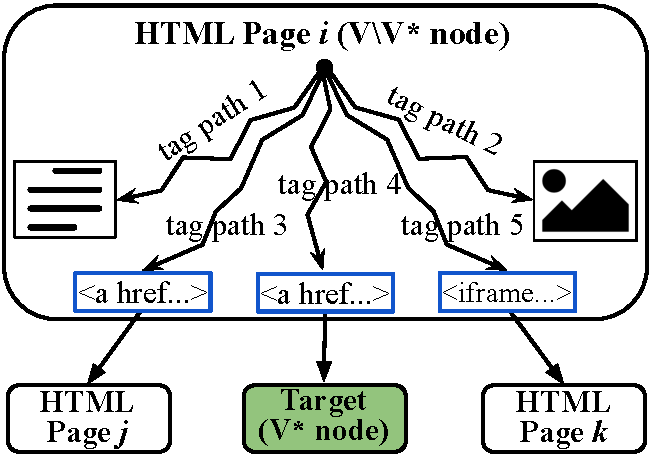
\includegraphics[width=0.65\linewidth]{plots/tag_paths_example.pdf}
	\caption{Tag paths in an HTML page}
	\label{fig:tag_paths_example}
\end{figure}

\begin{toappendix}
	Here is the full list of the 38 MIME types used to identify targets in 
	our implementation:

	\bigskip

	{\ttfamily\begin{tabular}{l}
			application/csv                                                           \\
			application/json                                                          \\
			application/msword                                                        \\
			application/octet-stream                                                  \\
			application/pdf                                                           \\
			application/rdf+xml                                                       \\
			application/rss+xml                                                       \\
			application/vnd.ms-excel                                                  \\
			application/vnd.ms-excel.sheet.macroenabled.12                            \\
			application/vnd.oasis.opendocument.presentation                           \\
			application/vnd.oasis.opendocument.spreadsheet                            \\
			application/vnd.oasis.opendocument.text                                   \\
			application/vnd.openxmlformats-officedocument.presentationml.presentation \\
			application/vnd.openxmlformats-officedocument.spreadsheetml.sheet         \\
			application/vnd.openxmlformats-officedocument.wordprocessingml.document   \\
			application/vnd.openxmlformats-officedocument.wordprocessingml.template   \\
			application/vnd.rar                                                       \\
			application/x-7z-compressed                                               \\
			application/x-csv                                                         \\
			application/x-gtar                                                        \\
			application/x-gzip                                                        \\
			application/xml                                                           \\
			application/x-pdf                                                         \\
			application/x-rar-compressed                                              \\
			application/x-tar                                                         \\
			application/x-yaml                                                        \\
			application/x-zip-compressed                                              \\
			application/yaml                                                          \\
			application/zip                                                           \\
			application/zip-compressed                                                \\
			text/comma-separated-values                                               \\
			text/csv                                                                  \\
			text/json                                                                 \\
			text/plain                                                                \\
			text/x-comma-separated-values                                             \\
			text/x-csv                                                                \\
			text/x-yaml                                                               \\
			text/yaml                                                                 \\
		\end{tabular}}
	\clearpage
\end{toappendix}
